\documentclass[12pt onesided letterpaper]{report}
\usepackage{graphicx}
\usepackage{sidecap}

\title{Skeuomorphism and the Mental Model}
\author{Kaitlyn Higa}
\date{October 30, 2012}
\maketitle


\begin{document}

\section*{Introduction}
Whether it is fueled by magic or specified down to the gear, everyone has some perception of how things function.  Simple mechanics, like those which dictate those that dictate how a can opener works, are easily seen by the user and can be readily visualized when recalled at.  However, when that physicality is abstracted and the material and virtual nuts and bolts are hidden away, the mechanics behind the function becomes less and less apparent.  Historically, cultures have created elaborate stories to explain the processes behind things that could not be explained, such as the mythological explanation of seasons through Persephone and Hades.  Ancient Greek culture created a believable, workable model of how the climate changes operated.  Similarly, in today’s virtual world, some functions are masked by an interface that mimics the way we as humans interact with the physical world.  This graphical principle is called direct manipulation.  Developers have come to include familiar albeit functionally unnecessary gestures and interfaces which have been classified as “skeuomorphic.” This would seem to suggest that inclusion of these skeuomorphic details help to foster rapport for such systems.  However, there is the question of how effective these skeuomorphic are in the usability of said systems, based upon how well the user can visualize how the product works.   By adding skeuomorphs, developers create a simulated mental model of how virtual systems work, but this does not affect usability.

\section*{Mental Models}
In his book, The Design of Everyday Things, Donald Norman describes the phenomenon of an individual’s concept of how a certain item should perform while being utilized.  He christens this concept a “mental model” and continues to demonstrate the importance of creating a product that constructs a correct mental model in the consumer’s mind.  This idea of synching the developer’s mental model to that of the user is crucial to the end user’s desire to utilize the product and subsequently, usage of the product.   These mental models are built upon the existing psychology materials and things or rather “affordances of objects.” \cite[~p. 11]  {norman02}  These affordances are defined as the “perceived and actual properties of a given object primarily those fundamental properties that determine just how the thing could possibly be used.” \cite[~p. 11]  {norman02}  Western doors open on a hinge horizontally, slots are to have things inserted into them, raised buttons are meant to be pressed, and doorknobs are meant to be turned.  In this, the mental model of the process of opening a door to one of the rooms in a residence hall on Loyola Marymount University’s campus can easily be envisioned.  Additionally, Norman brings up the fact that humans are very good at discerning what should work and what shouldn’t.  Exhibiting this photo below, he brings up how all persons immediately know that this design for a tandem bicycle is inoperable.  
\pagebreak
\begin{figure}[hb]
    \centering
    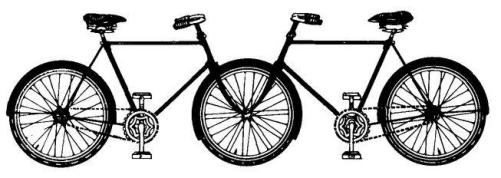
\includegraphics{bicycle}
    \caption{\emph{Carelman's Tandem "Convergent Bicycle"} featured in Norman's book. \cite[~p. 13]  {norman02}}
    
\end{figure}

In contrast Norman makes an example of the digital watch which has identical push buttons on the side, and elaborates on the futility of natural indications of how to complete a task such as changing the time.  Norman simply meets this undertaking by stating “There is no way to tell – no evident relationship between the operating controls and the functions, no constraints, no apparent mappings.”\cite[~p. 13]  {norman02}  Norman also expands his anecdote of an error-ridden telephone system that was installed at his university, describing the discontinuity between how the users think it should work and how it actually works.  He recalls the system’s complexity and how it was referred to as a “standing joke” It was so much of an issue that a computer program was written to ease the process of using the phone system.  The creators of the system had probably not taken the user of the phone while creating it, and subsequently created a failure of a system.  In order to create a successful system, the developer must always keep in mind the end user and their perceptions of how something works.

\section*{Skeuomorphism}
Skeuomorphism, a term which has come to mean a vestige which serves no useful purpose, remaining only as a decorative artifact, but was once useful or essential to the object in a previous time, is described by George Basalla in his book The Evolution of Technology.\cite[~p. 107-108]  {basalla88}  Such tangible, physical examples include the embossed rivet that covers the actual functional rivet underneath in a pair of jeans, the shutter sound on a digital camera, and decorative handles on pots.   These artifacts serve as decorative pointers to cultural trends, obsolete technologies, and even imitations of functional items.  The idea of skeuomorphism continues on into the virtual world, and is currently implemented in countless forms across all user interface platforms.  Microsoft word provides a “Print Layout” view of a document, in which the text appears on a white page, with a drop shadow on a grey background, simulating an actual piece of paper.  The Galaxy SIII phone requires a swipe to unlock the phone; the swipe itself triggers ripples similar to those created by water along with an accompanying splashing sound.  Many Android systems include a screen change swipe animation that zooms out to create a glass panel effect on the screen.  Even basic things such as the Save Icon being the obsolete floppy disk are considered skeuomorphs.  

\section*{Skeuomorphism, Popular Opinion, and the Mental Model}
Views on skeuomorphism and how it relates to the user interface vary from person to person.  Currently the most visible use of the concept is Apple’s integration of fluff graphics in their applications that mimic real world objects.  Their iCal application mimics an actual paper desk calendar, complete with leather binding and graphics that make it look as if pages have been torn out.  The bookshelves app features a wooden book shelf complete with varnished shelves and little books. The iCal and Bookshelves applications effectively create an environment where transition to the virtual is so familiar, it becomes identical.  Being this way, a user easily recognizes the functionality and creates a mental model of the virtual item flawlessly, by duplicating their mental model of the physical object and modifying it to become compatible with the virtual one.   Though one would think that such design choices would be optimal for creating a warm, familiar environment, there is a great dissent arising from the design community.  An article on Fast Company’s website details Austin Carr’s experience with disgruntled Apple developers who have expressed their contempt for the design, even going as far as to call it “visual masturbation.”\cite{carr12}  Many other bring up the issue of how much actual “design” work goes into such products if the physical model is simply replicated digitally.  These may seem trivial, but other issues do arrive through such designs.   Toggle bars, especially those in audio recording and modifying programs, are notoriously hard to control with a cursor or finger.  Though it will hopefully get you to approximately the correct area, nothing will be as concise as simply inputting a value via text.  Many others argue that such designs are created upon a concept that does not take into consideration the benefits of another design might afford.  The most heated comparison is to the upcoming Windows 8 operating system which features a minimalistic design with a significant lack of skeuomorphs.  Whether or not this design is successful is to be decided later with the release, but many are touting it to be superior to its Apple counterpart. 

\begin{SCfigure}
    \centering
    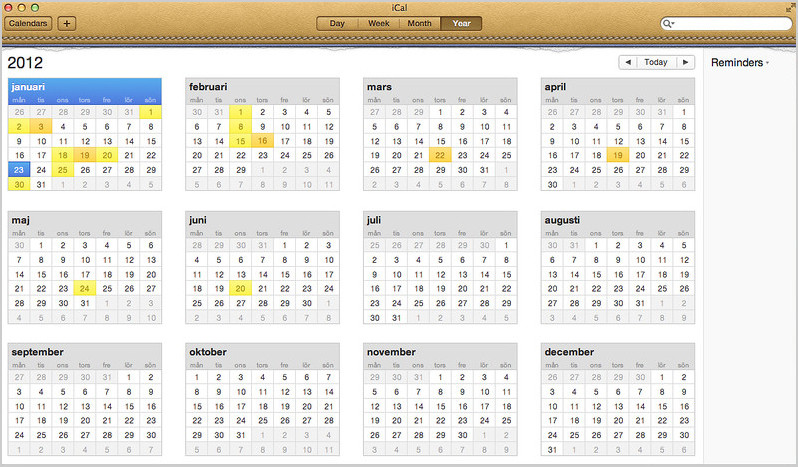
\includegraphics[scale = 0.5]{ical}
    \caption{Leather Stitching and Ripped pages of iCal. \cite{carr12}}
    
\end{SCfigure}
\pagebreak


However, not all skeuomorphic designs are hindering.  The idea of the drop shadow is greatly debated amongst designers but creates a psychological effect that cannot be doubted.  Though the drop shadow is merely darkened pixels with transparency, our brains have come to recognize that depth and the third dimension are implied.  It can be used to distinguish text from a background, show which windows hold preference over another, and create a “press-able” look for buttons.  With this, a user can apply affordances and quickly and efficiently create a mental model of perception and depth in this otherwise planar environment.  The user is then able to interact better, as the simulated three dimensions can be followed by a user who lives in a world containing three dimensions.  This skeuomorph enhances the experience of the user by helping them differentiate certain items on the display.  In regards to the alignment of the user’s and developer’s mental models, skeuomorphism creates a psychology, utilizing affordances that accurately make these conceptual models parallel.  In the case of iCal, a leather bound calendar that looks exactly like its physical counterpart immediately incites the function of a schedule keeper.  Skeuomorphs provide developers a way to ensure that their product is what their clients think they are getting. 


\section*{Conclusion}
In conclusion, there is no definite answer to the question of if the alignment of the user and developer mental models in the case of the benefits of creating skeuomorphic user interface designs.  The community remains as divided as the results of skeuomorphs themselves and a definite answer would result in countless rebuttals.  It seems essential that the mental models of both the user and the developer should be the same, but methods more efficient than creating skeuomorphs are argued.   As for usability of the interface, skeuomorphs do create harmony between mental models, but the ease of such features could be improved by non-skeuomorphic concepts. 

\begin{thebibliography}

\bibitem{basalla88}
  George Basalla.
  The Evolution of Technology.
  Cambridge University Press, Cambridge,
  1988.
  
\bibitem{norman02}
  Donald A. Norman.
  The Design of Everyday Things.
  Basic Books, New York,
  2nd Edition,
  2002.
  
\bibitem{carr12}
   Austin Carr.
   Will Apple’s Tacky Software-Design Philosophy Cause A Revolt?
   \url{http://www.fastcodesign.com/1670760/will-apples-tacky-software-design-philosophy-cause-a-revolt}
   2012
   

\end{thebibliography}


\end{document}

